%-----------------------------------------------------------------------------------------------------------------------------------------------%
%	The MIT License (MIT)
%
%	Copyright (c) 2015 Jan Küster
%
%	Permission is hereby granted, free of charge, to any person obtaining a copy
%	of this software and associated documentation files (the "Software"), to deal
%	in the Software without restriction, including without limitation the rights
%	to use, copy, modify, merge, publish, distribute, sublicense, and/or sell
%	copies of the Software, and to permit persons to whom the Software is
%	furnished to do so, subject to the following conditions:
%	
%	THE SOFTWARE IS PROVIDED "AS IS", WITHOUT WARRANTY OF ANY KIND, EXPRESS OR
%	IMPLIED, INCLUDING BUT NOT LIMITED TO THE WARRANTIES OF MERCHANTABILITY,
%	FITNESS FOR A PARTICULAR PURPOSE AND NONINFRINGEMENT. IN NO EVENT SHALL THE
%	AUTHORS OR COPYRIGHT HOLDERS BE LIABLE FOR ANY CLAIM, DAMAGES OR OTHER
%	LIABILITY, WHETHER IN AN ACTION OF CONTRACT, TORT OR OTHERWISE, ARISING FROM,
%	OUT OF OR IN CONNECTION WITH THE SOFTWARE OR THE USE OR OTHER DEALINGS IN
%	THE SOFTWARE.
%	
%
%-----------------------------------------------------------------------------------------------------------------------------------------------%


%============================================================================%
%
%	DOCUMENT DEFINITION
%
%============================================================================%

%we use article class because we want to fully customize the page and dont use a cv template
\documentclass[10.8pt,A4]{article}	


%----------------------------------------------------------------------------------------
%	ENCODING
%----------------------------------------------------------------------------------------

%we use utf8 since we want to build from any machine
\usepackage[utf8]{inputenc}		

%----------------------------------------------------------------------------------------
%	LOGIC
%----------------------------------------------------------------------------------------

% provides \isempty test
\usepackage{xifthen}

%----------------------------------------------------------------------------------------
%	FONT
%----------------------------------------------------------------------------------------

% some tex-live fonts - choose your own

%\usepackage[defaultsans]{droidsans}
%\usepackage[default]{comfortaa}
%\usepackage{cmbright}
%\usepackage[default]{raleway}
%\usepackage{fetamont}
%\usepackage[default]{gillius}
\usepackage[light,math]{iwona}
%\usepackage[thin]{roboto} 

% set font default
\renewcommand*\familydefault{\sfdefault} 	
\usepackage[T1]{fontenc}

% more font size definitions
\usepackage{moresize}		

\usepackage{fontawesome}

%----------------------------------------------------------------------------------------
%	PAGE LAYOUT  DEFINITIONS
%----------------------------------------------------------------------------------------

%debug page outer frames
%\usepackage{showframe}			


%define page styles using geometry
\usepackage[a4paper]{geometry}		

% for example, change the margins to 2 inches all round
\geometry{top=1cm, bottom=-.6cm, left=0.4cm, right=1cm} 	


%less space between header and content
\setlength{\headheight}{-5pt}		


%customize entries left, center and right
%\lhead{}
%\chead{ \small{Jan Küster  $\cdot$ Consultant and Software Engineer $\cdot$  Bremen, Germany  $\cdot$  \textcolor{sectcol}{\textbf{info@jankuester.com}}  $\cdot$ +49 176 313 *** **}}
%\rhead{}


%indentation is zero
\setlength{\parindent}{0mm}

%----------------------------------------------------------------------------------------
%	TABLE /ARRAY DEFINITIONS
%---------------------------------------------------------------------------------------- 

%for layouting tables
\usepackage{multicol}			
\usepackage{multirow}

%extended aligning of tabular cells
\usepackage{array}

\newcolumntype{x}[1]{%
>{\raggedleft\hspace{0pt}}p{#1}}%


%----------------------------------------------------------------------------------------
%	GRAPHICS DEFINITIONS
%---------------------------------------------------------------------------------------- 

%for header image
\usepackage{graphicx}

%for floating figures
\usepackage{wrapfig}
\usepackage{float}
%\floatstyle{boxed} 
%\restylefloat{figure}

%for drawing graphics		
\usepackage{tikz}				
\usetikzlibrary{shapes, backgrounds,mindmap, trees}
\usepackage{hyperref}

%----------------------------------------------------------------------------------------
%	Color DEFINITIONS
%---------------------------------------------------------------------------------------- 
\usepackage{transparent}
\usepackage{color}

%accent color
\definecolor{complcol}{RGB}{250,150,10}

%dark background color
\definecolor{bgcol}{RGB}{110,110,110}

%light background / accent color
\definecolor{softcol}{RGB}{225,225,225}

\definecolor{sectcol}{RGB}{0,120,150}


%============================================================================%
%
%
%	DEFINITIONS
%
%
%============================================================================%

% returns minipage width minus two times \fboxsep
% to keep padding included in width calculations
\newcommand{\mpwidth}{\linewidth-\fboxsep-\fboxsep}
	

%----------------------------------------------------------------------------------------
% 	ARROW GRAPHICS in Tikz
%----------------------------------------------------------------------------------------

% a six pointed arrow poiting to the left
\newcommand{\tzlarrow}{(0,0) -- (0.2,0) -- (0.3,0.2) -- (0.2,0.4) -- (0,0.4) -- (0.1,0.2) -- cycle;}	

% include the left arrow into a tikz picture
% param1: fill color
%
\newcommand{\larrow}[1]
{\begin{tikzpicture}[scale=0.58]
	 \filldraw[fill=#1!100,draw=#1!100!black]  \tzlarrow
 \end{tikzpicture}
}

% a six pointed arrow poiting to the right
\newcommand{\tzrarrow}{ (0,0.2) -- (0.1,0) -- (0.3,0) -- (0.2,0.2) -- (0.3,0.4) -- (0.1,0.4) -- cycle;}

% include the right arrow into a tikz picture
% param1: fill color
%
\newcommand{\rarrow}
{
\begin{tikzpicture}[scale=0.7]
	\filldraw[fill=sectcol!100,draw=sectcol!100!black] \tzrarrow
 \end{tikzpicture}
}

%----------------------------------------------------------------------------------------
%	custom sections
%----------------------------------------------------------------------------------------

% create a coloured box with arrow and title as cv section headline
% param 1: section title
%
\newcommand{\cvsection}[1]
{
\colorbox{sectcol}{\mystrut \makebox[1\mpwidth][l]{
\larrow{bgcol} \hspace{-8pt} \larrow{bgcol} \hspace{-8pt} \larrow{bgcol} \textbf{\textcolor{white}{\uppercase{#1}}}\hspace{4pt}
}}\\
}

% create a coloured arrow with title as cv meta section section
% param 1: meta section title
%
\newenvironment{metasection}[1] {
	\vspace{2pt}
	\begin{center}
		\textcolor{white}{\large{\uppercase{#1}}}\\
	\normalsize
	\parbox{0.7\mpwidth}{\textcolor{white}	\hrule}
}{\end{center}}

%----------------------------------------------------------------------------------------
%	 CV EVENT
%----------------------------------------------------------------------------------------

% creates a stretched box as cv entry headline followed by two paragraphs about 
% the work you did
% param 1:	event time i.e. 2014 or 2011-2014 etc.
% param 2:	event name (what did you do?)
% param 3:	institution (where did you work / study)
% param 4:	what was your position
% param 5:	some words about your contributions
%
\newcommand{\cvevent}[5]
{
\vspace{6pt}
	\begin{tabular*}{1\mpwidth}{p{0.45\mpwidth}  x {0.51\mpwidth}}
 	\textcolor{black}{\textbf{#2}} & \textcolor{complcol}{#3}, \textcolor{bgcol}{#1} 
	\end{tabular*}
	\\[3pt]
\vspace{-12pt}
\textcolor{softcol}{\hrule}
\vspace{6pt}
	\begin{tabular*}{0.5\mpwidth}{p{\mpwidth}}
\larrow{softcol}  #4 \\[6pt]
\larrow{softcol}  #5 \\[6pt]
	\end{tabular*}

}

\newcommand{\cveventmin}[4]
{
\vspace{6pt}
	\begin{tabular*}{1\mpwidth}{p{0.45\mpwidth}  x {0.51\mpwidth}}
 	\textcolor{black}{\textbf{#2}} & \textcolor{complcol}{#3}, \textcolor{bgcol}{#1} 
	\end{tabular*}
\vspace{3pt}
\textcolor{softcol}{\hrule}
\vspace{3pt}
	\begin{tabular*}{0.5\mpwidth}{p{\mpwidth}}
\larrow{softcol}  #4 \\[3pt]
	\end{tabular*}

}

\newcommand{\cveventuni}[7]
{
\vspace{6pt}
	\begin{tabular*}{1\mpwidth}{p{0.45\mpwidth}  x {0.51\mpwidth}}
 	\textcolor{black}{\textbf{#2}} & \textcolor{complcol}{#3}, \textcolor{bgcol}{#1} 
	\end{tabular*}
	\\[3pt]
\vspace{-12pt}
\textcolor{softcol}{\hrule}
\vspace{6pt}
	\begin{tabular*}{0.5\mpwidth}{p{\mpwidth}}
\larrow{softcol}  #4 \\[6pt]
\larrow{softcol}  #5 \\[6pt]
\larrow{softcol}  #6 \\[6pt]
\larrow{softcol}  #7 \\[6pt]
	\end{tabular*}

}


% creates a stretched box as 
\newcommand{\cveventmeta}[2]
{
	\mbox{\mystrut \hspace{87pt}\textit{#1}}\\
	#2
}

%----------------------------------------------------------------------------------------
% CUSTOM STRUT FOR EMPTY BOXES
%----------------------------------------- -----------------------------------------------
\newcommand{\mystrut}{\rule[-.3\baselineskip]{0pt}{\baselineskip}}

%----------------------------------------------------------------------------------------
% CUSTOM LOREM IPSUM
%----------------------------------------------------------------------------------------
\newcommand{\lorem}
{Lorem ipsum dolor sit amet, consectetur adipiscing elit. Donec a diam lectus.}


% use to vertically center content
% credits to: http://tex.stackexchange.com/questions/7219/how-to-vertically-center-two-images-next-to-each-other
\newcommand{\vcenteredinclude}[1]{\begingroup
\setbox0=\hbox{\includegraphics{#1}}%
\parbox{\wd0}{\box0}\endgroup}

% use to vertically center content
% credits to: http://tex.stackexchange.com/questions/7219/how-to-vertically-center-two-images-next-to-each-other
\newcommand*{\vcenteredhbox}[1]{\begingroup
\setbox0=\hbox{#1}\parbox{\wd0}{\box0}\endgroup}

%----------------------------------------------------------------------------------------
%	ICON-SET EMBEDDING
%---------------------------------------------------------------------------------------- 

% at this point we simplify our icon-embedding by simply referring to a set of png images.
% if you find a good way of including svg without conflicting with other packages you can
% replace this part
\newcommand{\icon}[3]{\makebox(#2, #2){\textcolor{#3}{\csname fa#1\endcsname}}}	%icon shortcut
\newcommand{\icontext}[4]{ 						%icon with text shortcut
	\vcenteredhbox{\icon{#1}{#2}{#4}} \vcenteredhbox{\textcolor{#4}{#3}}
}



%============================================================================%
%
%
%
%	DOCUMENT CONTENT
%
%
%
%============================================================================%
\begin{document}
\fcolorbox{white}{white}{\begin{minipage}[c][0.95\textheight][t]{0.69\linewidth}


%---------------------------------------------------------------------------------------
%	TITLE HEADLINE
%----------------------------------------------------------------------------------------
\vspace{-3pt}
% use this for multiple words like working titles etc.
%\hspace{-0.25\linewidth}\colorbox{bgcol}{\makebox[1.5\linewidth][c]{\hspace{46pt}\HUGE{\textcolor{white}{\uppercase{M.Sc. Jan Küster}} } \textcolor{sectcol}{\rule[-1mm]{1mm}{0.9cm}} \parbox[b]{5cm}{   \large{ \textcolor{white}{{IT Consultant}}}\\
% \large{ \textcolor{white}{{JS Fullstack Engineer}}}}
%}}

% use this for single words, e.g. CV or RESUME etc.
\colorbox{bgcol}{\makebox[\mpwidth][c]{\HUGE{\textcolor{white}{\uppercase{Steve Sim}} } \textcolor{sectcol}}}

%----------------------------------------------------------------------------------------
%	HEADER IMAGE
%----------------------------------------------------------------------------------------


%\hspace{-1.6cm}
%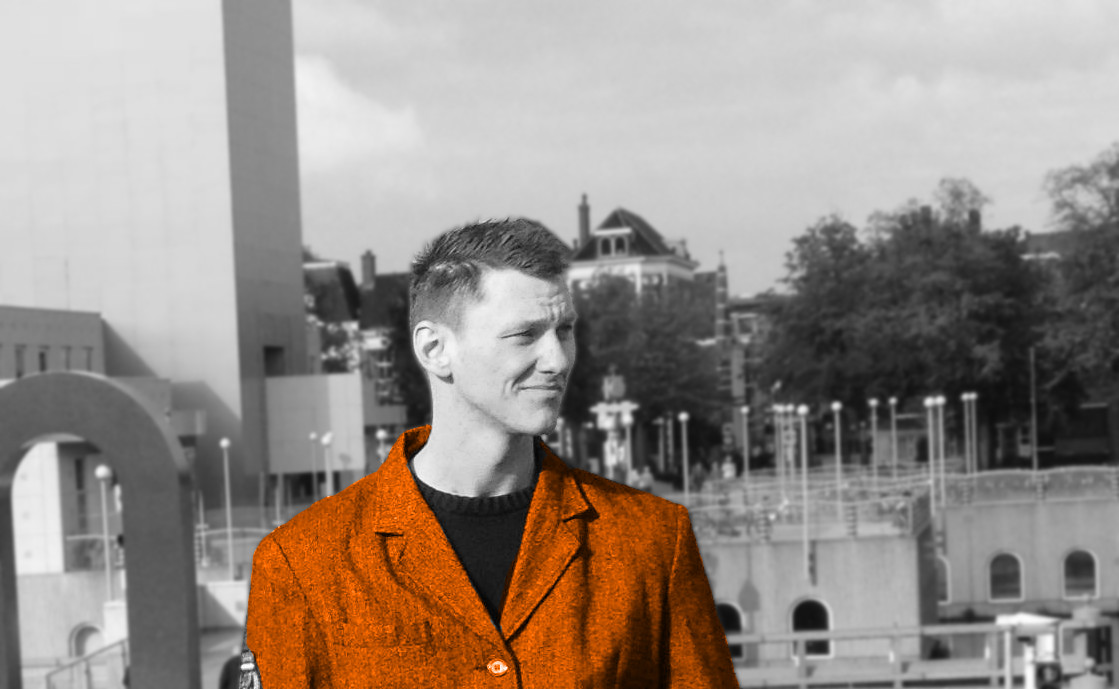
\includegraphics[trim= 0 250 0 270,clip,width=1\linewidth+3.1cm]{myfoto.jpg}	%trimming relative to image size!

%---------------------------------------------------------------------------------------
%	SUMMARY
%----------------------------------------------------------------------------------------

%============================================================================%
%
%	CV SECTIONS AND EVENTS (MAIN CONTENT)
%
%============================================================================%

%---------------------------------------------------------------------------------------
%	STATUS
%----------------------------------------------------------------------------------------
\cvsection{About me}
\\[1pt]
{An enthusiastic, diligent and curious computing graduate with over 4 years of knowledge and experiences focused on Software Engineering and Information Technology.
Confident and proficient in working within teams and projects during academic and personal time.
Currently experienced and passionate on full stack development, data mining and data management.
\\[5pt]
}
\vspace{10pt}
%---------------------------------------------------------------------------------------
%	Achievements
%----------------------------------------------------------------------------------------
\cvsection{Achievements}
\cveventmin{November 2018}{Dynamo challenge}{Bournemouth University}{Representing Bournemouth university on an inter-university challenge, working on set of challenges by IBM , to present an innovative solution for coming future of AI, and received high valued feedback for the proposed solution.}

\cveventmin{2016-2017}{Global Talent Programme}{Bournemouth University}{Credited for developing innovative future-ready global talent and attributes such as leadership, effective communication skills and innovative problem solving and thinking.}

\cveventmin{April 2016}{Computing in Business Week}{Bournemouth University}{Successfully led the team to achieve 2nd place academically when designing prototype time-sheet system for Kingfishers.}
\vspace{10pt}
%===========================================================================================

%---------------------------------------------------------------------------------------
%	EXPERIENCE
%----------------------------------------------------------------------------------------
\cvsection{Experience}

\cvevent{Jan 2018 - Jun 2018}{Front End developer}{Met Office}{Invented and shared a web component using Angular that can be used by other projects in the Office, aim to reduce development time for other projects.} {Project leading, as well as gathering requirements, designing, implementing and testing the web component.}

%\textcolor{softcol}{\hrule}


%\cvevent{2014 - 2016}{IT Consultant for IBM XPages and Notes Domino}{We4IT GmbH Bremen}{Realize projects in XPages and We4IT Aveedo, monitor project status, conduct reports}{Integrated Camunda BPMN engine and BPMN.IO modeler in We4IT Aveedo}


%\textcolor{softcol}{\hrule}


\cvevent{Jul 2017 - Jun 2018}{IT practitioner} {Met Office}{Worked with a critical project that aims to deliver weather warnings to the general public.}{Main responsible includes manual testing, writing/running automated tests, documentation and implementation of some front and back end features.}

%\textcolor{softcol}{\hrule}

%
\cvevent{2016}{Computing in Business Week}{Bournemouth University}{Performed a 4 day project to design an interactive prototype system for Kingsfisher.}{Topics included customer contracts, change management, controlling, operational tasks.}

%\textcolor{softcol}{\hrule}

\vspace{10pt}
%---------------------------- -----------------------------------------------------------
%	EDUCATION SECTION
%--------------------------------------------------------------------------------------
\cvsection{Academic Qualifications}

\cveventuni{2015 - 2019}{Computing Framework - 2:1}{Bournemouth University}{Studied Data mining, System software modelling and Human Factors.}{Developed Final year project supervision tools for supervisors and students using Angular framework, Microsoft Graph and Azure.}
{Studied into advanced modern computing such as IoT, Cisco networking with routers and switches, Agile project management and Application development using Java and Android.}
{Studied into modern computing such as virtual machines, usability and systems software, programming in Java and relational database using mySQL.}


%\textcolor{softcol}{\hrule}


\cvevent{2013 - 2015}{A-Level}{Poole High School}{Studied and mastered 3 subjects : Computing, Information Technology and Psychology.}{Learned to code in C\# and VB.NET, IT project management as well as understanding human interactive behaviours.}

\end{minipage}}%
\fcolorbox{white}{sectcol}{\begin{minipage}[c][0.95\textheight][t]{0.33\linewidth}
\LARGE{
\vspace{5pt}
\begin{metasection}{Quick Info}
\begin{center}
\hspace{0.5cm}\begin{tabular}{@{}l@{}}
	\icontext{Linkedin}{14}{\hspace{0.1cm}linkedin.com/in/steve-sim1997}{white}\\[2pt]
	\icontext{Github}{14}{\hspace{0.1cm}github.com/Saims123}{white}\\[2pt]
	\icontext{Send}{14}{\hspace{0.1cm}stevesim@hotmail.com}{white}\\[2pt]
    \icontext{Mobile}{14}{\hspace{0.1cm}07516548663}{white}\\
\end{tabular}
\end{center}

\end{metasection}
%----------------------------------------------------------------------------------------
%	META SECTION
%----------------------------------------------------------------------------------------
\begin{metasection}{Fields}

\begin{center}
\begin{tabular}{@{}l@{}}
    \icontext{CodeFork}{13}{\hspace{0.2cm}Agile Project Management}{white}\\[2pt]
    \icontext{Database}{13}{\hspace{0.5cm}Data Management}{white}\\[2pt]
    \icontext{Code}{13}{\hspace{0.5cm}System Modelling}{white}\\[2pt]
    \icontext{Code}{13}{\hspace{0.5cm}Software Development}{white}\\[2pt]
    \icontext{CommentsO}{13}{\hspace{0.5cm}Software Testing}{white} \\[2pt]
    \icontext{User}{13}{\hspace{0.5cm}Humans Factors}{white}\\
\end{tabular}
\end{center}
\end{metasection}

\begin{metasection}{Key strength}
\begin{center}
    \hspace{-1cm} \begin{tabular}{@{}l@{}}
    \icontext{Search}{14}{\hspace{0.5cm}Analytical}{white} \\[2pt] 
    \icontext{User}{14}{\hspace{0.5cm}Team Player}{white}\\[2pt]
    \icontext{Wrench}{14}{\hspace{0.5cm}Problem Solving}{white}\\[2pt]
    \icontext{LightbulbO}{14}{\hspace{0.5cm}Critical Thinker}{white}\\[2pt]
    \icontext{Flash}{14}{\hspace{0.5cm}Fast Learner}{white}\\[2pt]
    \icontext{Gears}{14}{\hspace{0.5cm}Flexible}{white}\\
\end{tabular}
\end{center}
\end{metasection}

\begin{metasection}{Technical skills}

\textcolor{white}{

\begin{tabular}{c c}
\icontext{Code}{14}{Typescript}{white} & \icontext{Code}{14}{NodeJS}{white}  \\[6pt]
\icontext{Code}{14}{C\#}{white} & \icontext{Code}{14}{Java}{white} \\[6pt]
\icontext{Database}{14}{mySQL}{white} & \icontext{Database}{14}{MongoDB}{white} \\[6pt]\icontext{CodeFork}{14}{Git}{white} & \icontext{Connectdevelop}{14}{AWS}{white} \\[6pt]
\icontext{Buysellads}{14}{Angular > 4}{white} & \icontext{Windows}{14}{.NET}{white}
\end{tabular}

}
\end{metasection}

\begin{metasection}{Tools}
\begin{center}
    \icontext{Code}{14}{Visual Studio}{white}
    \icontext{Code}{14}{Intellij}{white}\\[6pt]
    \icontext{CodeFork}{14}{SourceTree}{white}
    \icontext{Terminal}{14}{Terminal}{white}\\[6pt]
    \icontext{Github}{14}{GitHub}{white}
\end{center}

\end{metasection}

\begin{metasection}{Certification}
    \textcolor{white}{
    \begin{tabular}{c c}
        \icon{Certificate}{13}{white} &  {Dynamo Challenge}\\
        \icon{Certificate}{13}{white} & {Global Talent Programme}\\
        \icon{Certificate}{13}{white} & {Cisco CCNA Router \& Switch}
    \end{tabular}
}

\end{metasection}

\begin{metasection}{Operating Systems}

\textcolor{white}{\LARGE{
\icon{Windows}{24}{white}
\icon{Linux}{24}{white}}}

\end{metasection}
}


\vspace{12pt}

\end{minipage}}
%
%
%
%	DOCUMENT END
%
%
%
%============================================================================%
\end{document}